\section{第一节}

\begin{frame}
    \frametitle{本节上机概要}

    本节课讲述的内容：
    \begin{itemize}
        \item Python的安装和使用。
        \item 虚拟环境的安装和使用。
        \item Python的基本语法，以及Numpy的基本使用。
    \end{itemize}
    如果你确信你已经掌握了这些内容，你不必听这节课，下一次上机再来听就行了。

    本节默认同学们的水平接近零基础。

    \alert{讲义很简略，是提示，不是详细说明。你一定要在我讲述和演示操作的时候跟着操作，一定要确保自己确实会操作！}

    \alert{如果哪里听不懂或跟不上，务必及时提出！}

\end{frame}

\begin{frame}
    \frametitle{关于这门课的编程需求}

    用到的99\%编程语言是Python3。

    基本不需要GPU，CPU能够解决99\%的作业问题了。即使不能，我们也会提供GPU资源。

    当然，如果你有自己的GPU，那自然是欢迎使用的，能为作业提速不少。

\end{frame}

\subsection{Python和虚拟环境}

\begin{frame}
    \frametitle{Python简介}

    Python是一个简单易学的编程语言，广泛应用于多种领域，有蓬勃的第三方生态，所以在多个领域有着重要的地位。AI领域也不例外，Python是AI领域的主流编程语言之一（其余还有R、C/C++、Julia等）。

    与C/C++不同，Python是一种解释型语言，不需要编译，直接运行即可。不过也因此需要特定的解释器来执行Python代码。

    Python官网：\url{https://www.python.org/}

    \alert{不要立即从上述官网下载安装Python！}

\end{frame}

\begin{frame}
    \frametitle{虚拟环境简介}

    正因为Python的第三方生态非常丰富，所以在不同的项目中可能需要安装不同的第三方库，甚至同一个库的不同版本。为了避免不同项目之间的依赖冲突，我们需要隔离不同项目的依赖。另，分发项目时，也需要让其余人能够复现项目的环境，以便能够正确运行项目。

    故而，引入\textbf{虚拟环境}。

    虚拟环境一般可以隔离不同的：
    \begin{itemize}
        \item 编译器或解释器版本；
        \item 第三方库及其版本；
        \item 系统级别依赖。
    \end{itemize}

\end{frame}

\begin{frame}
    \frametitle{虚拟环境管理工具}

    一般情况下，我们会使用一些工具来管理虚拟环境，常见的有：venv、conda（Anaconda、Miniconda、Mamba、Micromamba等）、pixi等。

    这节课，我们主要聚焦于conda。

    理由：开山鼻祖，库多而全，技术成熟，文档完善，使用广泛。

    缺陷：慢，且不能100\%隔离系统级别依赖，也不能100\%复现环境，且环境和项目分离。不过在这门课基本够用了。

\end{frame}

\begin{frame}
    \frametitle{安装conda}

    比较建议安装简单的Miniconda，比较轻量。有兴趣的同学可以安装Micromamba，速度更快。

    \url{https://docs.conda.io/projects/conda/en/23.11.x/user-guide/install/download.html}

    \alert{conda是免费软件。如果你发现你需要付费，那说明你被骗了！}

    \textbf{务必在安装过程中勾选“添加到PATH环境变量”选项！}否则会非常麻烦地需要手动添加环境变量。

    可以使用命令 \mintinline{bash}|conda --version| 来验证安装是否成功。

\end{frame}

\begin{frame}
    \frametitle{换源（非常重要！！！）}

    由于网络原因，conda和PyPI默认的官方源在国内访问速度非常慢，甚至无法访问。因此，强烈建议将默认源替换为国内的镜像源，以提高安装和更新包的速度。

    不要用北大源，会变得不幸。

    清华源：\url{https://mirrors.tuna.tsinghua.edu.cn/}

    在这两个网站上找anaconda和PyPI，按照说明进行换源配置即可。换源配置完成后，你就可以享受更快的安装速度了。

\end{frame}

\begin{frame}
    \frametitle{conda环境的使用}

    创建环境：\mintinline{bash}|conda create -n myenv python=3.10|

    进入环境：\mintinline{bash}|conda activate myenv|

    退出环境：\mintinline{bash}|conda deactivate|

    删除环境：\mintinline{bash}|conda remove -n myenv --all|

    你的命令行通常会显示当前激活的环境名称，以便你知道你正在使用哪个环境。
    \begin{figure}
        \centering
        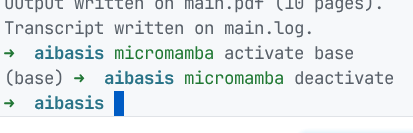
\includegraphics[width=0.5\textwidth]{env.png}
    \end{figure}

\end{frame}

\subsection{Python简介}

\begin{frame}
    \frametitle{pip的使用}

    pip是Python的包管理工具，可以用来安装和管理Python包。conda环境中也可以使用pip来安装包。这是因为conda太慢了，环境一大，解析起来就更慢了，所以我们通常使用pip来安装包。

    安装包：\mintinline{bash}|pip install package_name|

    升级包：\mintinline{bash}|pip install --upgrade package_name|

    卸载包：\mintinline{bash}|pip uninstall package_name|

    列出已安装的包：\mintinline{bash}|pip list|

\end{frame}

\begin{frame}
    \frametitle{pip导出和安装环境}

    导出到文件：\mintinline{bash}|pip freeze > requirements.txt|

    从文件装包：\mintinline{bash}|pip install -r requirements.txt|

    交作业时请一定要提供这个requirements.txt文件，以便助教能够复现你的环境。\textbf{因未提交该文件而导致环境无法复现的，可能造成扣分！}

\end{frame}

\begin{frame}
    \frametitle{关于文本编辑器}

    较为著名的Python IDE：JB Pycharm。问题：臃肿。

    Python自带的IDE：Python IDLE。问题：功能过于简单，且不太好用。

    建议使用轻量级的文本编辑器，如VS Code、Vim（NeoVim）、Notepad（Notepad++）、Sublime Text、Atom等。这些编辑器提供了丰富的插件和功能，可以提高编程效率。

\end{frame}

\begin{frame}
    \frametitle{关于Code}

    个人推荐VS Code，功能强大且免费，社区活跃，插件丰富，支持多种编程语言和工具，使用也并不像Vim一样过于困难。

    \url{https://code.visualstudio.com/}，选择System Installer版本（而非User Installer版本），安装时勾选“Add to PATH”选项。

    \alert{VS Code是免费软件。如果你发现你需要付费，那说明你被骗了！}

\end{frame}

\begin{frame}
    \frametitle{配置Code}

    安装以下插件：Python，Python Debugger，Pylance。

    英语苦手的同学可以安装Chinese (Simplified) Language Pack for Visual Studio Code插件来将VS Code界面翻译成中文。

    你会在界面右下角见到一个“选择解释器”的选项。如果你的系统里有Python解释器或你创建了虚拟环境，你就会在这里看到系统解释器或虚拟环境的解释器。你可以选择其中一个作为VS Code的默认解释器，这样在VS Code中运行Python代码时就会使用这个解释器了。

    mamba用户稍复杂些，见相关资料。

\end{frame}

\begin{frame}
    \frametitle{Python基本使用}

    在命令行中输入 \mintinline{bash}|python| ，就进入了Python的交互式环境，可以直接输入Python代码进行测试和调试。

    输入 \mintinline{bash}|exit()| 或按Ctrl+D可以退出Python交互式环境。

    如欲运行某代码code.py文件，可以在命令行中输入 \mintinline{bash}|python code.py| 来执行该文件中的代码。

    若你安装了Code，你可以在Code中打开code.py文件，然后按F5或点击运行按钮来运行该文件中的代码。

    你可以在代码的行号处打断点，然后按F5或点击调试按钮来调试代码，这样就可以逐行执行代码，查看变量的值，分析代码的执行流程了。

\end{frame}

\begin{frame}[fragile]
    \frametitle{Python语法}

    与C++这种静态类型语言不同，Python是一种动态类型语言。虽然依然需要遵循先声明、再使用的原则，但不需要声明变量的类型，变量的类型会在运行时自动推断。
    \begin{minted}{python}
x = 10 # 实际上这就是个声明，声明x并赋值。
print(x)  # 输出: 10
x = "Hello, World!"
print(x)  # 输出: Hello, World!
    \end{minted}

\end{frame}

\begin{frame}
    \frametitle{Python的基本类型}

    虽然Python是动态类型语言，但它是强类型的。“动态类型”指的是某一变量的类型在运行时确定，换言之，不同时间同一变量的类型可以不同；但一个确定的时间点上，某一变量的类型是确定的，不会同时具有多种类型。

    Python的内置类型包括：int、float、str、bool、list、tuple、dict、set、None等。强制类型转换也在Python中是支持的，例如 \mintinline{python3}{int("123")} 会将字符串 "123" 转换为整数 123，无需调用 \mintinline{cpp}|std::stoi| 这样的函数，这是Python字符串处理的一个优势。
    
    Python3.8以后允许写类型注释，即 \mintinline{python}|x: int = 10| ，但这只是注释，并不会真正限制变量的类型。Pylance插件会根据类型注释提供极其有限的类型检查和智能提示。

\end{frame}

\begin{frame}[fragile]
    \frametitle{Python的变量运算}

    所以在C++中的加减乘除（单双目）、与或非、大小等、赋值在Python中也适用，但Python还支持一些额外的运算符，如幂运算符 \mintinline{python3}{**} 、取模运算符 \verb|%| 、整除运算符 \mintinline{python3}{//} 等。

    需要注意的是，在Python中，5/2==2.5，而不是2。这是因为Python中的除法运算符 \mintinline{python3}{/} 总是返回一个浮点数结果。如果你想要像C++一样得到整数结果，可以使用整除运算符 \mintinline{python3}{//} ，即5//2==2。

    Python没有自增自减运算符，也没有取地址运算符。这是因为Python没有指针。

    Python用井号 \mintinline{python3}{\#} 来表示注释，直接在代码行前加 \mintinline{python3}{\#} 即可。

\end{frame}

\begin{frame}[fragile]
    \frametitle{Python条件分支}

    Python中的条件语句使用 \mintinline{python3}{if} 、\mintinline{python3}{elif} 和 \mintinline{python3}{else} 来实现，功能和使用基本上与C++中的条件语句相同，但Python使用冒号和缩进来表示代码块，而不是花括号。\textbf{Python中的缩进重要且严格，必须使用一致的缩进方式（通常是4个空格）来表示代码块，否则会导致语法错误。}

    \begin{minted}{python}
if x == 2: # 必须换行并缩进
    print("x is 2")
elif x > 2:
    print("x is greater than 2")
else:
    print("x is less than 2")
    \end{minted}

\end{frame}

\begin{frame}[fragile]
    \frametitle{Python循环}

    Python中循环有两种： \mintinline{python3}{while} 循环（和C++中的while类似）和 \mintinline{python3}{for} 循环（和C++中的range-for类似）。
    \begin{minted}{python3}
while x > 0:
    print(x)
    x -= 1
    \end{minted}
\end{frame}

\begin{frame}[fragile]
    \frametitle{Python迭代}

    Python的for循环可以直接迭代任何可迭代对象，如列表、字符串、字典等，非常方便。
    \begin{minted}{python3}
for i in range(5):  # range(5)生成一个可迭代对象，包含0到4的整数
    print(i)
for i in [1, 2, 3]:  # 直接迭代一个列表
    print(i)
for char in "Hello":  # 直接迭代一个字符串
    print(char)
    \end{minted}
    需要说明的是， \mintinline{python3}|range(5)| 实际上是一个生成器对象，指的是0到5的整数序列（不包含5），而不是一个列表。
\end{frame}

\begin{frame}[fragile]
    \frametitle{复合数据类型}
    Python中的复合数据类型包括列表（list）、元组（tuple）、字典（dict）和集合（set）。这些数据类型可以存储多个值，并且支持各种操作，如添加、删除、访问等。

    Python的这些复合数据类型都是可以直接打印的，且打印出来的格式非常友好，方便调试和展示。

    \begin{minted}{python3}
l: list[int] = [1, 2, 3]  # 列表，有序可更改
t: tuple[int, int, int] = (1, 2, 3)  # 元组，有序不可更改
d: dict[str, int] = {"a": 1, "b": 2}  # 字典，键值对，无序可更改
s: set[int] = {1, 2, 3}  # 集合，无序不重复可更改
    \end{minted}

\end{frame}

\begin{frame}[fragile]
    \frametitle{复合数据类型的操作}

    操作类似C++的STL。以list为例：
    \begin{minted}{python3}
x = l[0]  # 访问元素
l[0] = 10  # 修改元素
l.append(4)  # 添加元素
l.remove(2)  # 删除元素
l.sort()  # 排序
l.reverse()  # 反转
l.clear()  # 清空
l.insert(1, 5)  # 在索引1处插入元素5
    \end{minted}

\end{frame}

\begin{frame}[fragile]
    \frametitle{切片}

    切片（slicing）是Python中一种非常强大的功能，可以用来获取列表、元组、字符串等序列的一部分。切片的语法是 \mintinline{python3}{sequence[start:stop:step]} ，其中 \mintinline{python3}{start} 是起始索引， \mintinline{python3}{stop} 是结束索引（不包含）， \mintinline{python3}{step} 是步长（可以为负数）。

    切片会返回一个新的序列，原序列不受影响。

\end{frame}

\begin{frame}
    \frametitle{推导式}

    列表推导式（list comprehension）是一种简洁的语法，可以用来创建新的列表。它的基本语法是 \mintinline{python3}{[expression for item in iterable if condition]} ，其中 \mintinline{python3}{expression} 是生成新列表元素的表达式， \mintinline{python3}{item} 是迭代器中的每个元素， \mintinline{python3}{iterable} 是一个可迭代对象， \mintinline{python3}{condition} 是一个可选的条件表达式。

    实际上，推导式不仅可以用来生成列表，还可以用来生成其他类型的集合，如字典推导式（dictionary comprehension）和集合推导式（set comprehension）。但因为推导式会对可读性造成一定的影响，所以不建议使用过度复杂的推导式。

    推导式的本质实际上是循环。

\end{frame}

\begin{frame}[fragile]
    \frametitle{函数}

    Python中函数的定义使用 \mintinline{python3}{def} 关键字，后跟函数名和参数列表。例如：
    \begin{minted}{python3}
def add(a: int, b: int) -> int: # 这里的三个int都是类型注释，实际并不限制参数和返回值的类型。
# def add(a, b):  # 也可以不写类型注释
    return a + b
    \end{minted}
    Python中的函数参数可以有默认值，也可以是可变参数（*args）或关键字参数（**kwargs）。函数也可以返回多个值，实际上是返回一个元组。

\end{frame}

\begin{frame}
    \frametitle{可变参数和关键字参数}

    可变参数指的是函数参数的数量不固定，可以接受任意数量的参数。换言之，args是一个元组，但可以在传参时不显式地传入一个元组，而是直接传入多个参数，Python会自动将它们打包成一个元组。
    
    关键字参数类似，指的是函数参数以键值对的形式传递，可以接受任意数量的键值对参数。换言之，kwargs是一个字典，同样可以不显式地传入一个字典，而是直接传入多个键值对参数。

\end{frame}

\begin{frame}[fragile]
    \frametitle{面向对象}

    Python是一种面向对象的编程语言，支持类和对象的概念。你可以使用 \mintinline{python3}{class} 关键字来定义一个类，然后创建该类的实例（对象）来使用它。例如：
    \begin{minted}{python3}
class Person:
    def __init__(self, name: str, age: int):
        self.name = name  # 属性
        self.age = age
    def greet(self): # 方法
        print(f"Hello, my name is {self.name} and I am {self.age} years old.")
    \end{minted}

\end{frame}

\begin{frame}[fragile]
    \frametitle{类的实例化}

    可以通过创建 \mintinline{python3}{Person} 类的实例来使用上文中提到的类，例如：
    \begin{minted}{python3}
person1 = Person("Alice", 30)
person1.greet()  # 输出: Hello, my name is Alice and I am 30 years old.
    \end{minted}
    故而我们刚刚这种调用 \mintinline{python3}|l.append(4)| 的方式，其实就是在调用list类的append方法。

\end{frame}

\begin{frame}[fragile]
    \frametitle{类的常用属性}

    一般的，要实现一个类，我们往往需要实现以下常用属性：
    \begin{itemize}
        \item \mintinline{python3}|__init__(self, ...)|：构造函数，用于初始化对象的属性。
        \item \mintinline{python3}|__str__(self)|：字符串表示方法，用于定义对象的字符串表示形式，方便打印和调试。
        \item \mintinline{python3}|__repr__(self)|：对象表示方法，用于定义对象的详细表示形式，通常在调试时使用。
        \item \mintinline{python3}|__eq__(self, other)|：相等性比较方法，用于定义对象之间的相等性比较逻辑。
    \end{itemize}
    当然，你也可以根据需要实现其他的特殊方法，如 \mintinline{python3}|__add__(self, other)| 用于定义对象之间的加法操作， \mintinline{python3}|__len__(self)| 用于定义对象的长度等。Python的运算符重载实际上都是通过实现这些特殊方法来实现的。

\end{frame}

\begin{frame}[fragile]
    \frametitle{数据类}

    Python 3.7引入了数据类（dataclass）的概念，相当于简单的结构体。Python会自动实现其常用方法。

    \begin{minted}{python3}
from dataclasses import dataclass

@dataclass # 装饰器，告诉Python这是一个数据类
class Point:
    x: float
    y: float
    \end{minted}

\end{frame}

\begin{frame}[fragile]
    \frametitle{模块和包}

    \begin{minted}{python3}
import math  # 相当于#include <cmath>;
from math import sqrt  # 相当于#include <cmath>和using std::sqrt;
from math import *  # 相当于#include <cmath>和using namespace std;
    \end{minted}
    需要注意的是，第三种方式可能会导致命名冲突，因此不建议使用这种方式导入模块。

    允许为模块或函数指定别名，例如 \mintinline{python3}{import numpy as np} ，这样就可以使用 \mintinline{python3}{np} 来代替 \mintinline{python3}{numpy} ，使代码更简洁。
\end{frame}

\subsection{Numpy简介}

\begin{frame}
    \frametitle{Numpy简介}

    Numpy是Python中一个非常重要的科学计算库，提供了高效的多维数组对象和丰富的数学函数，可以用来进行各种数值计算和数据分析。Numpy的核心数据结构是ndarray（n维数组），它可以存储大量的数据，并且支持各种操作，如切片、广播、线性代数等。

    我们的第一次作业需要用到Numpy做手写梯度回传，所以建议同学们提前安装好Numpy库，并且熟悉一下它的基本用法。

    安装略，见前文pip的使用。

\end{frame}

\begin{frame}[fragile]
    \frametitle{Numpy的基本使用}

    导入Numpy库： \mintinline{python3}|import numpy as np| 。一般不会把该别名改成其他的，这已经成为了一个约定俗成的习惯。

    Numpy最重要的对象是ndarray，可以通过 \mintinline{python3}{np.array()} 函数来创建一个ndarray。例如：
    \begin{minted}{python3}
import numpy as np
a = np.array([1, 2, 3])  # 创建一个一维数组
b = np.array([[1, 2], [3, 4]])  # 创建一个二维数组
    \end{minted}

\end{frame}

\begin{frame}[fragile]
    \frametitle{向量化操作}

    Numpy的一个重要特性是支持向量化操作，即可以对整个数组进行操作，而不需要使用循环。这使得代码更加简洁和高效。

    这包括三项内容：
    \begin{itemize}
        \item 广播（broadcasting）：当对不同形状的数组进行操作时，Numpy会自动进行广播，使得它们具有相同的形状。
            \item 通用函数（ufuncs）：Numpy提供了一些通用函数，可以对数组进行元素级的操作，如 \mintinline{python3}{np.add()} 、\mintinline{python3}{np.multiply()}等。
        \item 切片（slicing）：Numpy支持对数组进行切片操作，可以获取数组的一部分或修改数组的某些元素。
    \end{itemize}

\end{frame}

\begin{frame}[fragile]
    \frametitle{实例：快速操作数组}

    现在要对数组进行Leaky ReLU。传统的做法是利用列表推导式或循环，但这样效率较低。利用Numpy的向量化操作，我们可以直接对整个数组进行操作，运行起来比循环和列表推导式更快。

    \begin{minted}{python3}
import numpy as np
def leaky_relu(x):
    return np.where(x > 0, x, 0.01 * x)
x = np.array([-1, 0, 1, 2, 3])
y = leaky_relu(x)
print(y)  # 输出: [-0.01  0.    1.    2.    3.  ]
    \end{minted}

\end{frame}

\begin{frame}[fragile]
    \frametitle{实例：通用函数}

    除了 \mintinline{python3}|np.where| 这样的通用函数外，Numpy还提供了许多其他通用函数，如 \mintinline{python3}|np.add| 、\mintinline{python3}|np.multiply|等。这些函数可以对数组进行元素级的操作，从而避免使用循环来逐个元素进行操作。例如：
    \begin{minted}{python3}
import numpy as np
a = np.array([1, 2, 3])
b = np.array([4, 5, 6])
c = np.add(a, b)  # 对应元素相加
d = np.multiply(a, b)  # 对应元素相乘
print(c)  # 输出: [5 7 9]
print(d)  # 输出: [ 4 10 18]
    \end{minted}

\end{frame}

\begin{frame}[fragile]
    \frametitle{切片}

    Numpy支持对数组进行切片操作，和Python内置的切片语法是一样的，但返回的是原数组，不是拷贝，所以修改切片会修改原数组。

    \begin{minted}{python3}
import numpy as np
a = np.array([1, 2, 3, 4, 5])
print(a[1:4])  # 输出: [2 3 4]
print(a[:3])   # 输出: [1 2 3]
print(a[2:])   # 输出: [3 4 5]
    \end{minted}

\end{frame}

\begin{frame}[fragile]
    \frametitle{广播}
    广播是Numpy中一个非常强大的功能，当对不同形状的数组进行操作时，Numpy会自动进行广播，使得它们具有相同的形状。广播会导致数组的维数增加。
    \begin{minted}{python3}
import numpy as np
a = np.array([1, 2, 3])
b = np.array([[1], [2], [3]])
c = a + b  # 广播a和b，使它们具有相同的形状
print(c)  # 得到一个3x3的数组
    \end{minted}

\end{frame}

\begin{frame}
    \frametitle{Numpy练习}

    试着对一个ndarray实现：
    \begin{itemize}
        \item ReLU
        \item Leaky ReLU
        \item Sigmoid
        \item Tanh
    \end{itemize}
    并对其进行反向传播（即求导）。

    该练习不参与考核，但强烈建议同学们完成，以便更好地理解Numpy的使用和神经网络中的激活函数及其导数。

\end{frame}